\documentclass[beamer=true]{standalone}
\usepackage{preamblesnotes}

\begin{document}
\settitle{全內反射及應用\\Total internal reflection and application}{光學第三課(I)}{周末班}

\begin{frame}{球體的折射Refraction of sphere}
    \begin{figure}
        \centering
        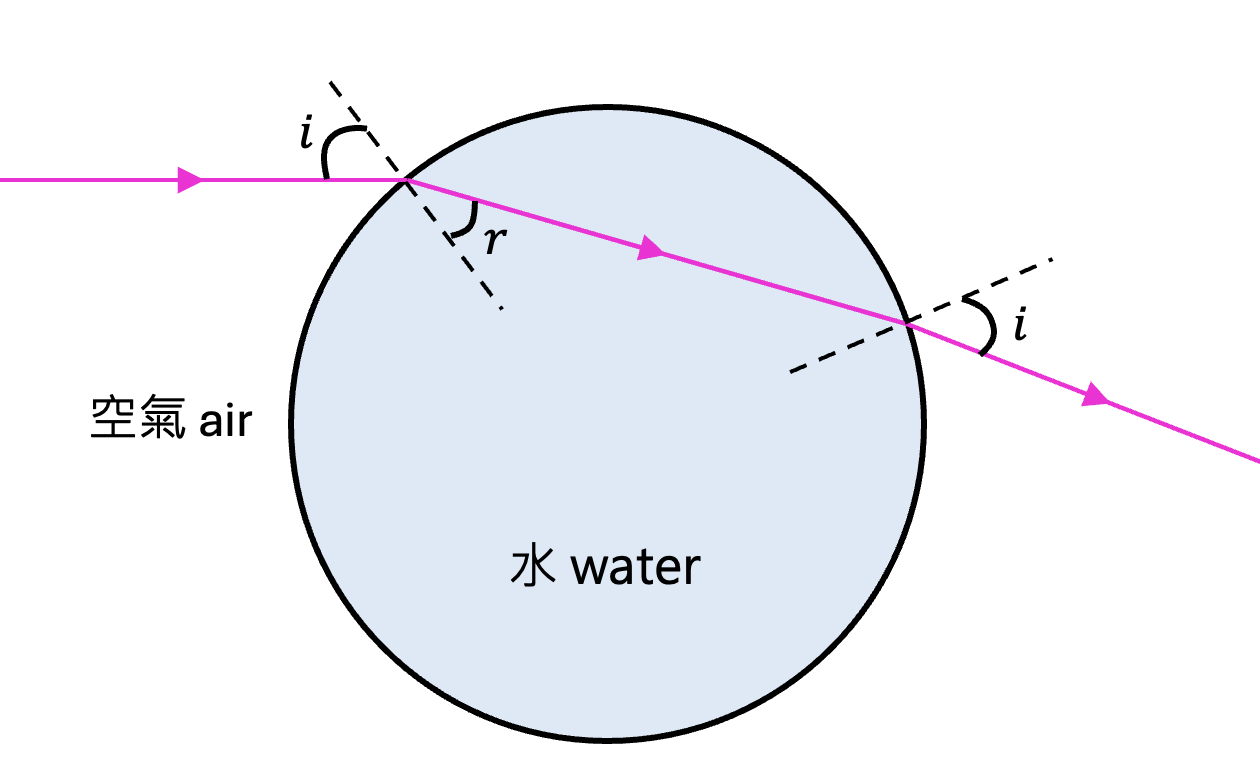
\includegraphics[width=0.45\linewidth]{assets/2980192839123.png}
        
    \end{figure}

    \begin{figure}
        \centering
        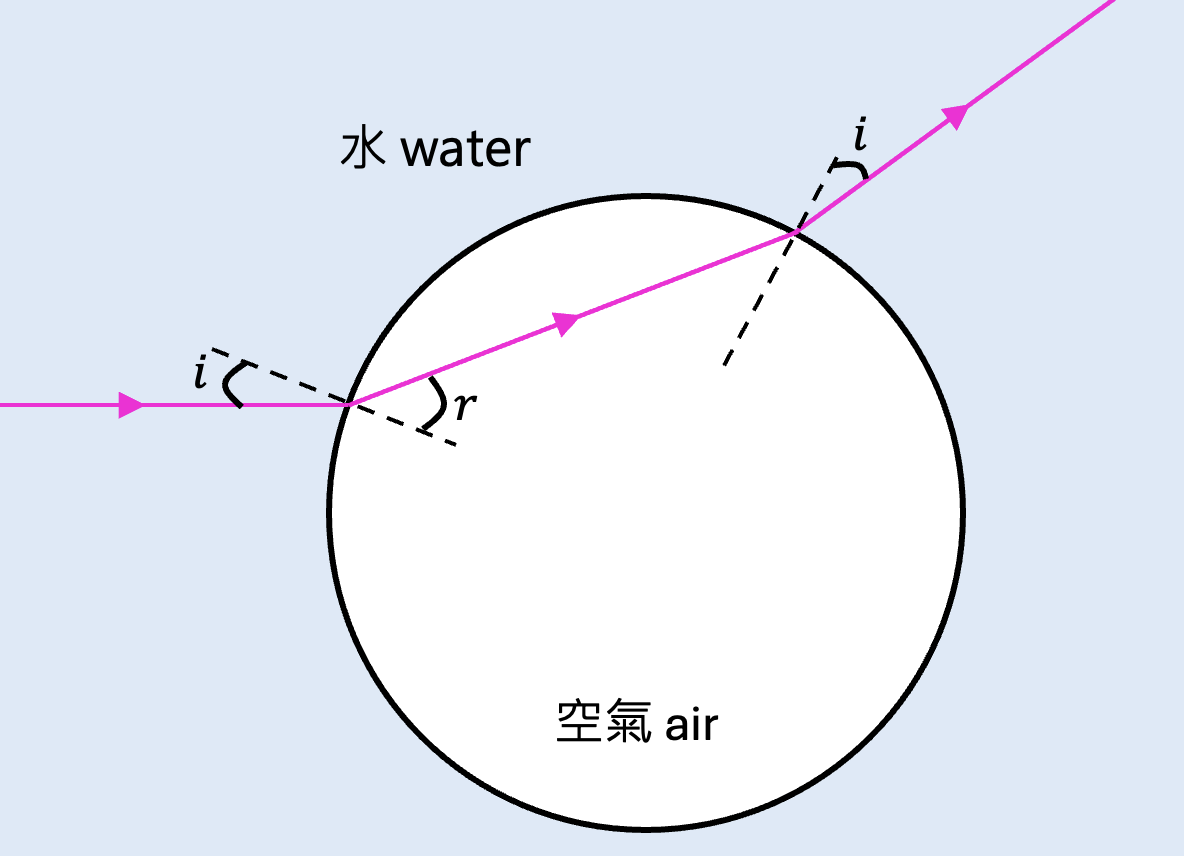
\includegraphics[width=0.45\linewidth]{assets/e12080481291d.png}
    \end{figure}
\end{frame}

% semi circle???



\begin{frame}{表觀深度 Apparent depth}
    \begin{figure}
        \centering
        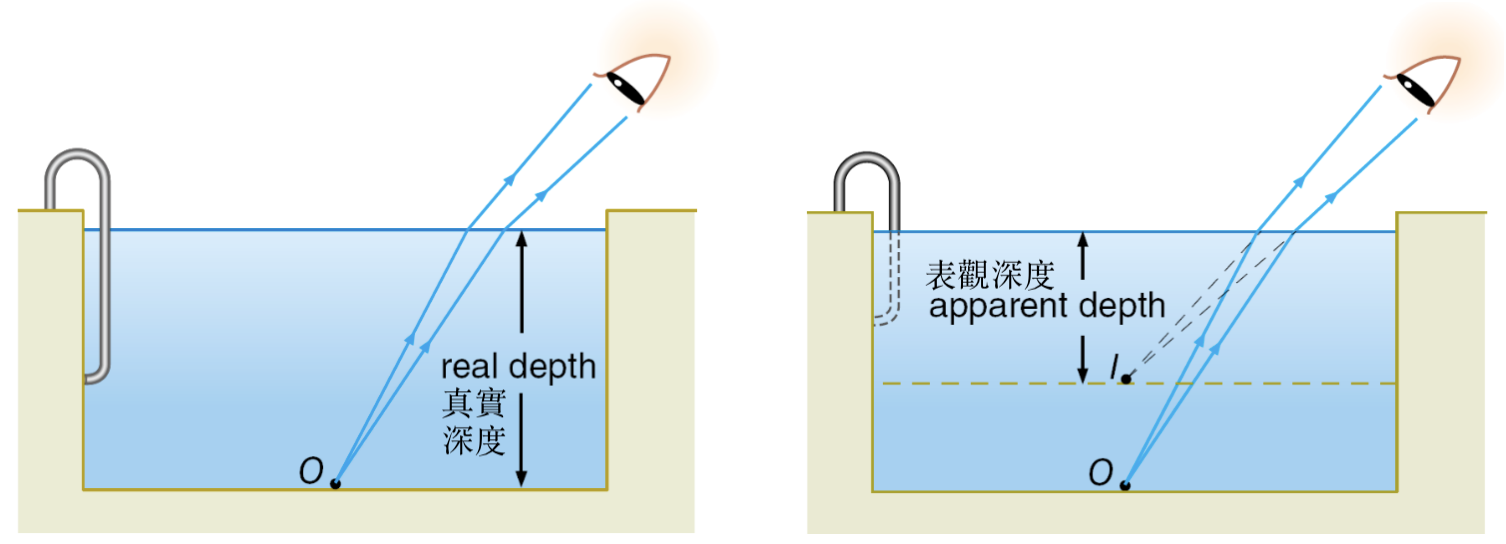
\includegraphics[width=0.9\linewidth]{assets/djoqwidjqwid213131.png}
    \end{figure}
\end{frame}


\begin{frame}{表觀深度 Apparent depth}
    \begin{columns}
        \column{.6\textwidth}
        \begin{itemize}
        \setlength{\itemsep}{.6em}
            \item 由於光的折射,觀察到的表觀深度會有所不同。\\ Due to refraction of light, there is apparent depth observed.
        \end{itemize}
        \column{.4\textwidth}
        \begin{figure}
            \centering
            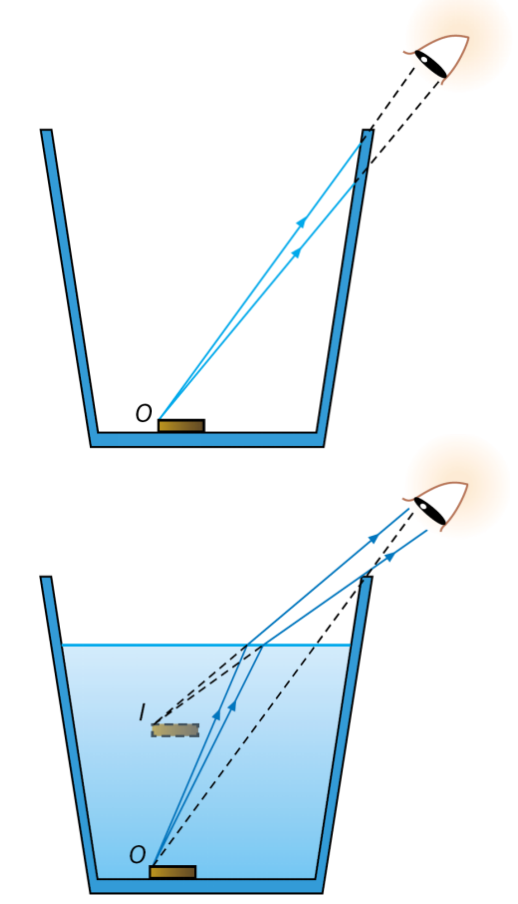
\includegraphics[width=.8\linewidth]{assets/q8ud9823du9n32d832.png}
            
            
        \end{figure}
    \end{columns}
\end{frame}

\begin{frame}{表觀深度 Apparent depth}
\begin{itemize}
    \item 對於在空氣中觀察的觀察者來說,水中的表觀深度小於實際深度。\\Apparent depth in water is less than the real depth for an observer in air.
\end{itemize}
    \begin{figure}
        \centering
        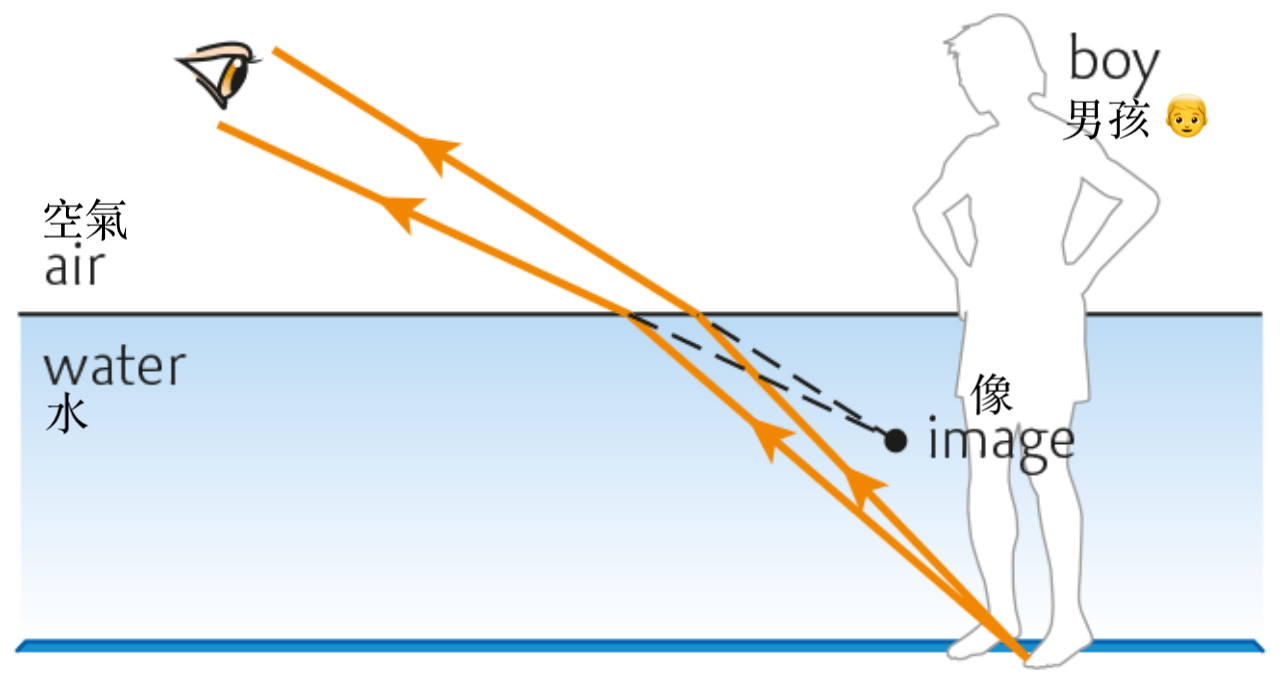
\includegraphics[width=0.75\linewidth]{assets/98398379879728dd.png}
        
        
    \end{figure}
\end{frame}

\begin{frame}{表觀深度 Apparent depth}
    \begin{itemize}
        \item 對於在水中觀察的觀察者來說,空氣中的表觀深度大於實際深度。\\Apparent depth in air is greater than the real depth for an observer in water.
    \end{itemize}
    \begin{figure}
        \centering
        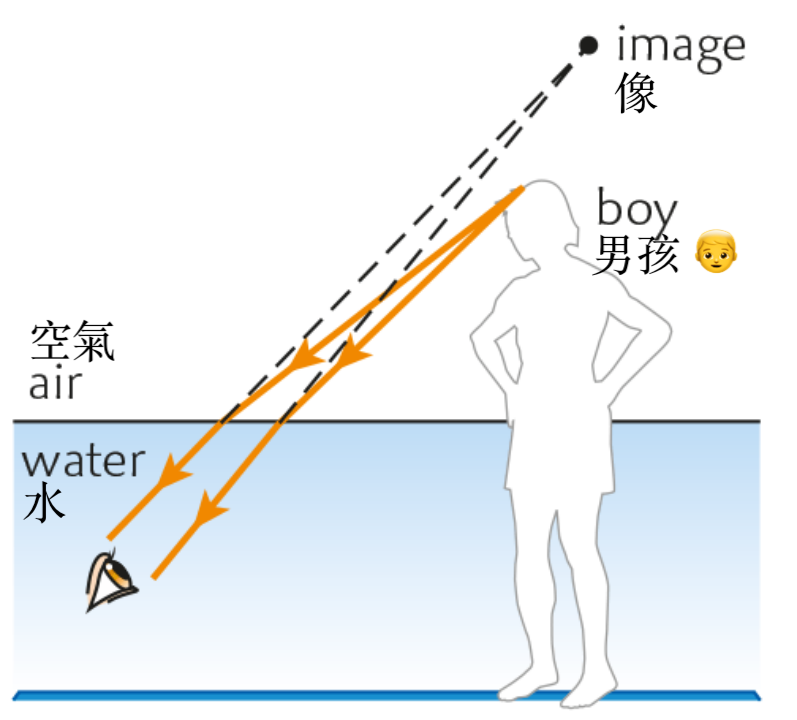
\includegraphics[width=0.5\linewidth]{assets/d9832u.png}
    \end{figure}
    
\end{frame}




\begin{frame}{全內反射Total internal reflection}
    \begin{figure}
        \centering
        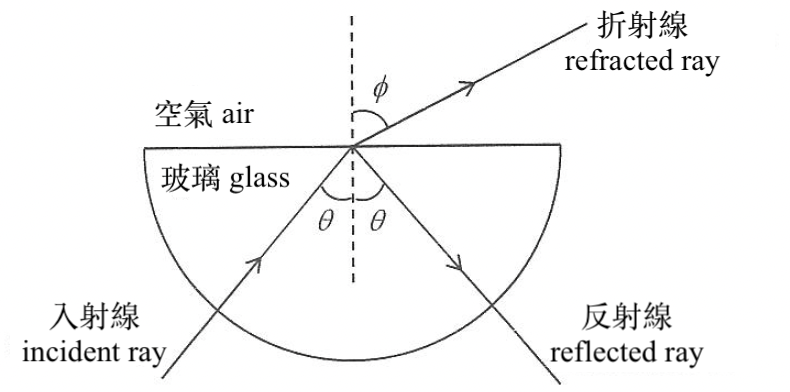
\includegraphics[width=0.6\linewidth]{assets/dqdwqdddd212.png}
        
        
    \end{figure}
\end{frame}

\begin{frame}{全內反射Total internal reflection}
    \begin{itemize}
        \item 隨著入射角 $\theta$ 逐漸增加,越來越多的光線被反射。\\As the incident angle $\theta$ gradually increases, more and more rays are reflected.
    \end{itemize}\medskip
    \begin{figure}
        \centering
        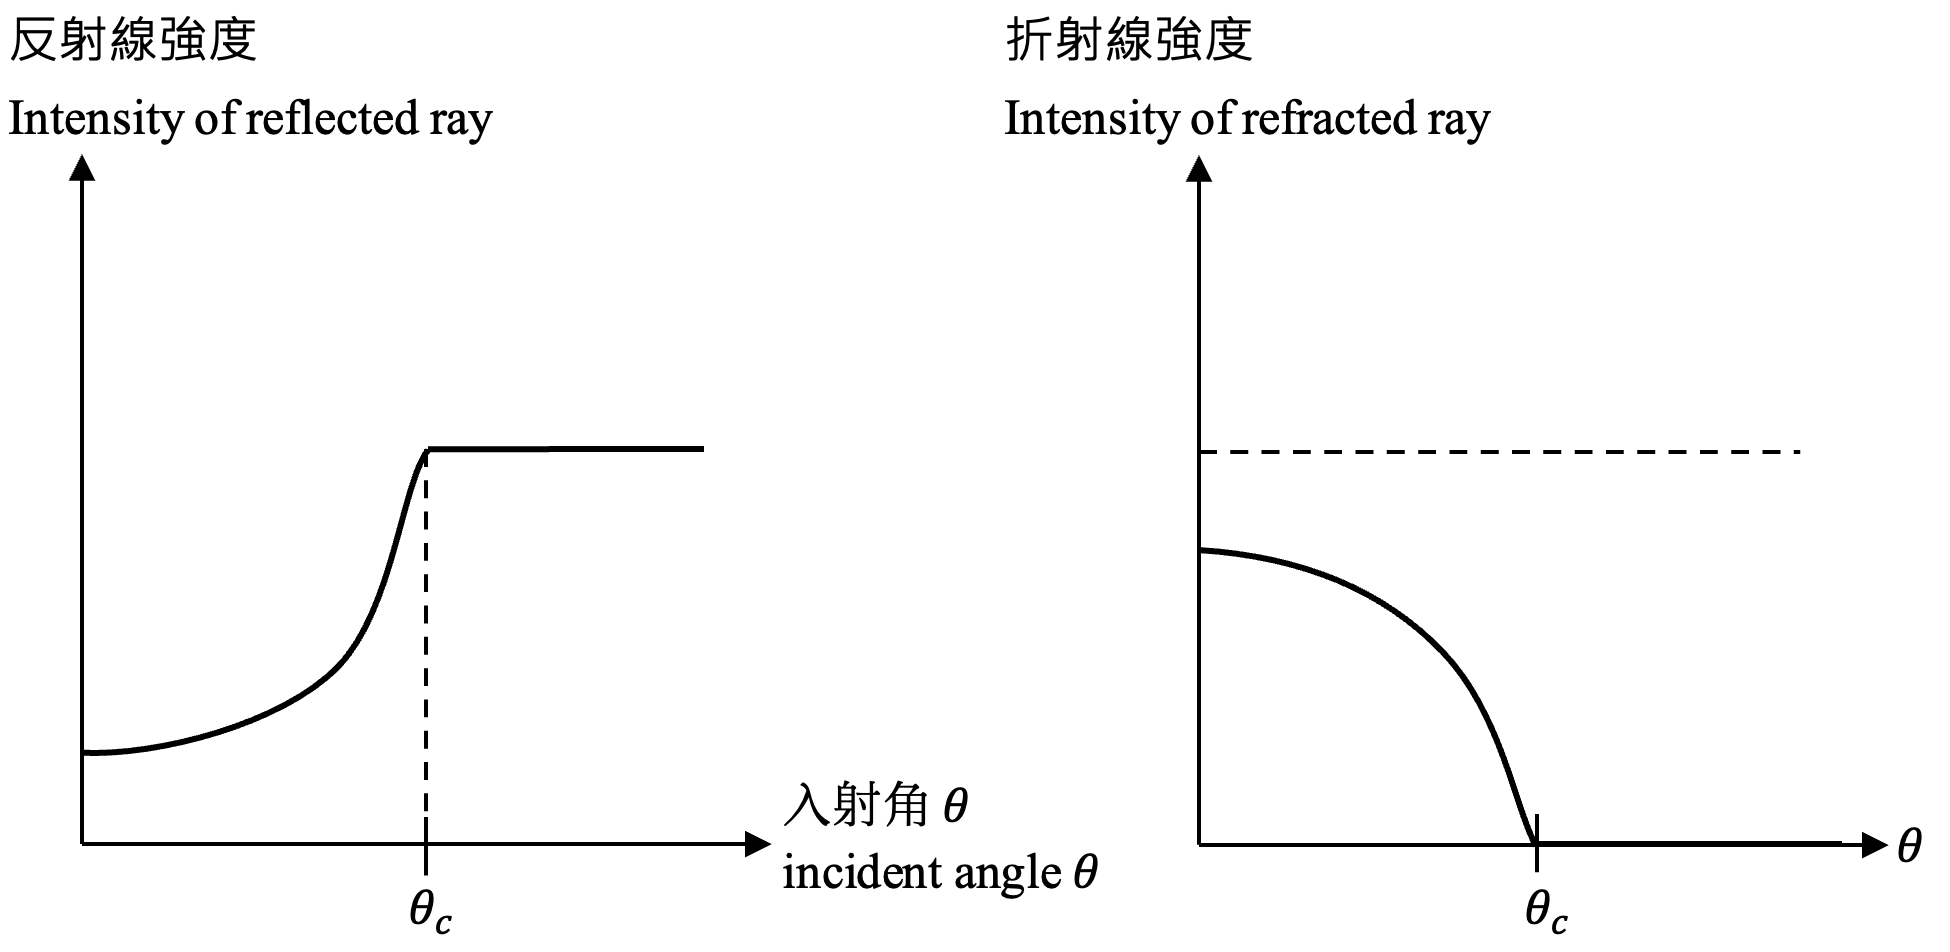
\includegraphics[width=0.9\linewidth]{assets/jd929828un2n32.png}
        
        
    \end{figure}
\end{frame}

\begin{frame}{全內反射Total internal reflection}
    \begin{figure}
        \centering
        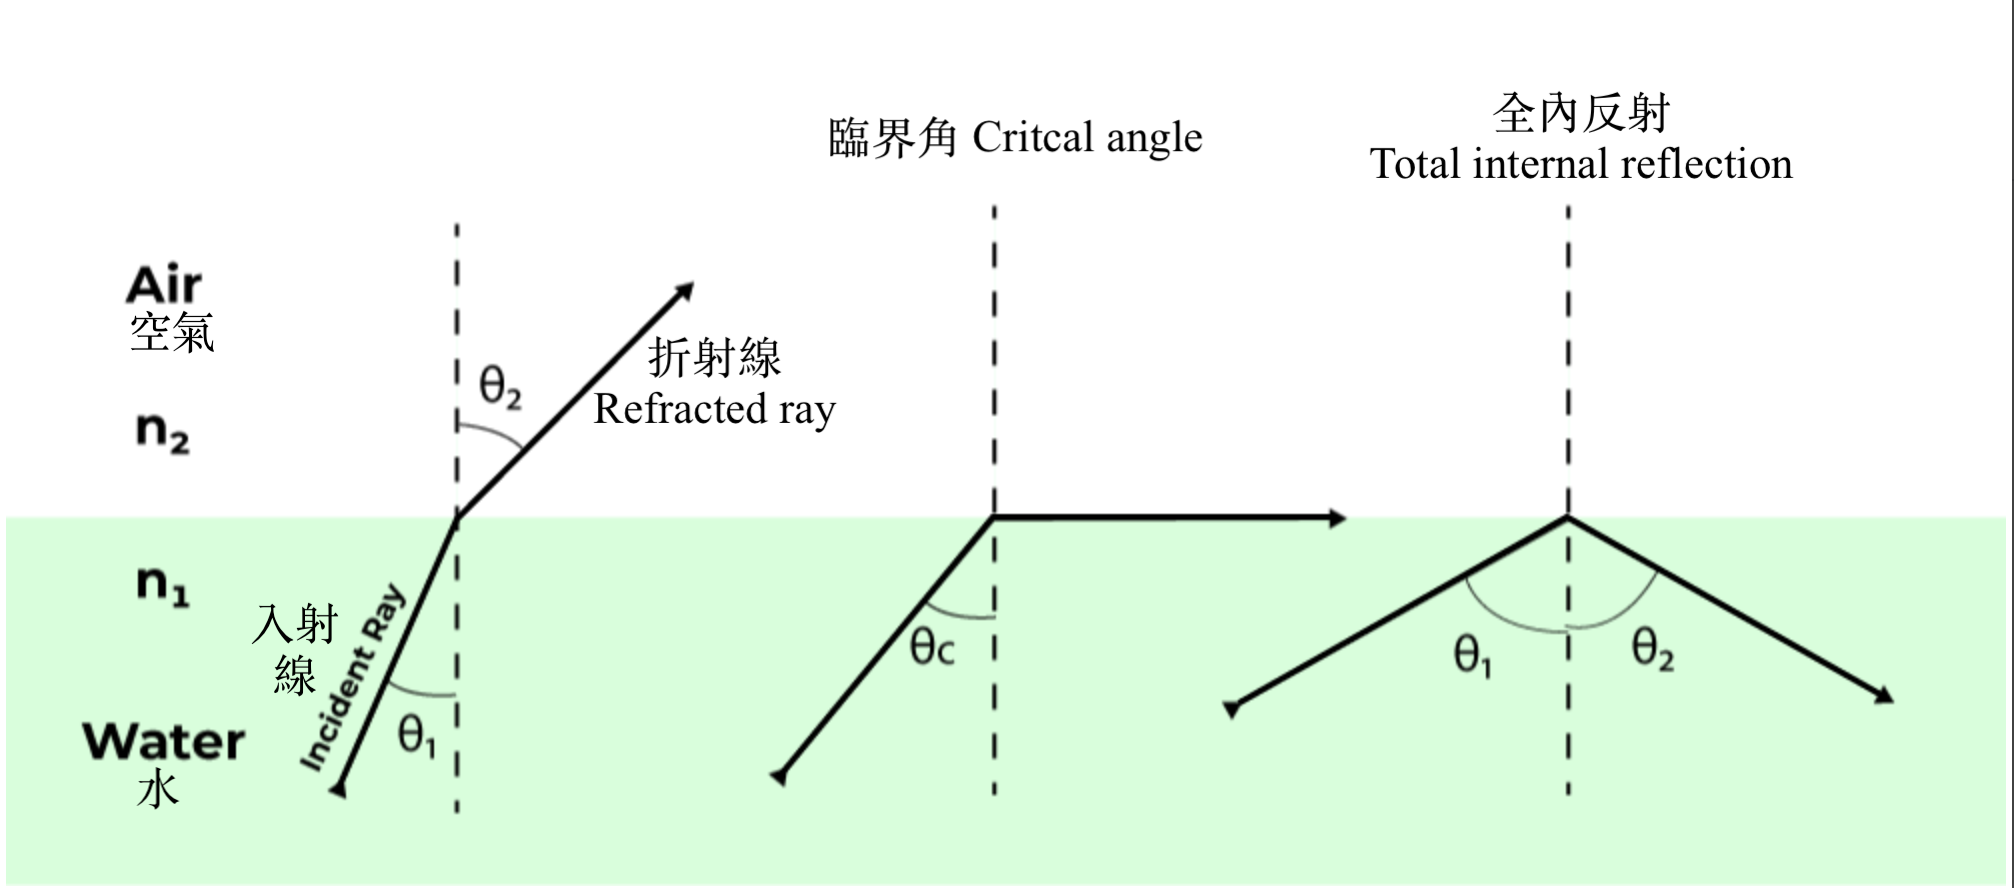
\includegraphics[width=1\linewidth]{assets/2839274194872184age.png}
    \end{figure}
\end{frame}

\begin{frame}{全內反射Total internal reflection}
    \begin{itemize}
        \item 介質的臨界角 $\theta_c$ 是介質中光線的入射角,使得在另一介質的折射角為\dg{90}。\\The critical angle $\theta_c$ of a medium is the incident angle of a light ray in the medium such that the refracted angle in another medium is \dg{90}.
        \item \fbox{$\dfrac{n_1}{n_2}=\dfrac{\sin\theta_c}{\sin 90^\circ}\quad\Rightarrow\quad \theta_c=\sin^{-1}\left(\dfrac{n_1}{n_2}\right)$}
    \end{itemize}
    \begin{figure}
        \centering
        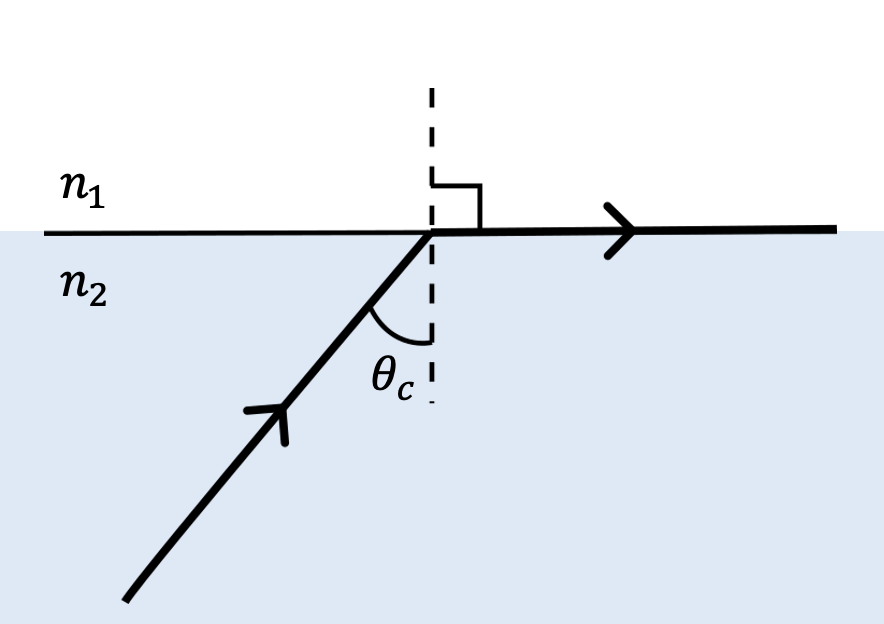
\includegraphics[width=0.4\linewidth]{assets/dd209i32.png}
    \end{figure}
    
\end{frame}

\begin{eg}
    下圖顯示光線穿過玻璃方塊其中一角的路徑。入射角$\theta$是多少?\\The diagram below shows the path of a light ray passing through the corner of a rectangular glass block. What is the angle of incidence $\theta$?
    \begin{figure}
       \raggedleft
        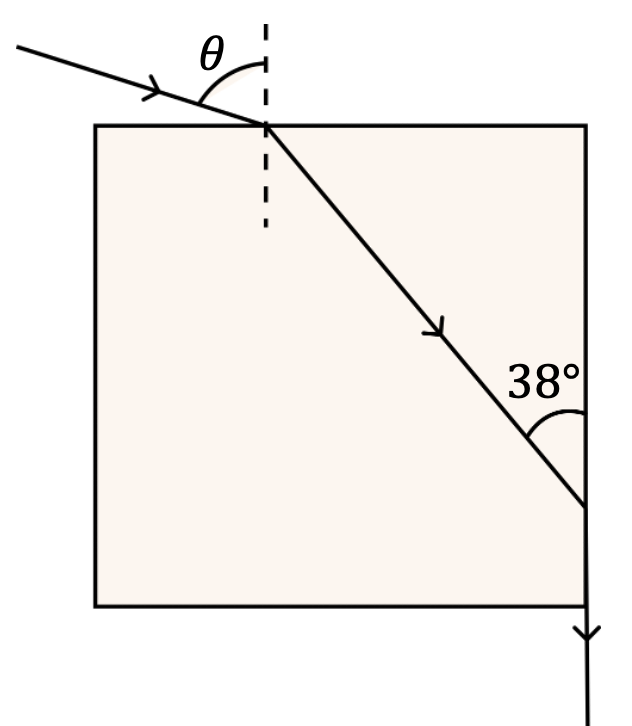
\includegraphics[width=0.35\linewidth]{assets/oij12i21.png}
    \end{figure}
\end{eg}

\begin{eg}
一條光線以入射角\dg{50}從空氣進入介質X。已 知$X$的臨界角為\dg{50}。求在$X$中的折射角。\\A ray of light travels in air and enters a medium $X$ at an angle of incidence \dg{50}. Given that the critical angle of $X$ is \dg{50}. Calculate the angle of refraction.
    \begin{figure}
        \raggedleft
        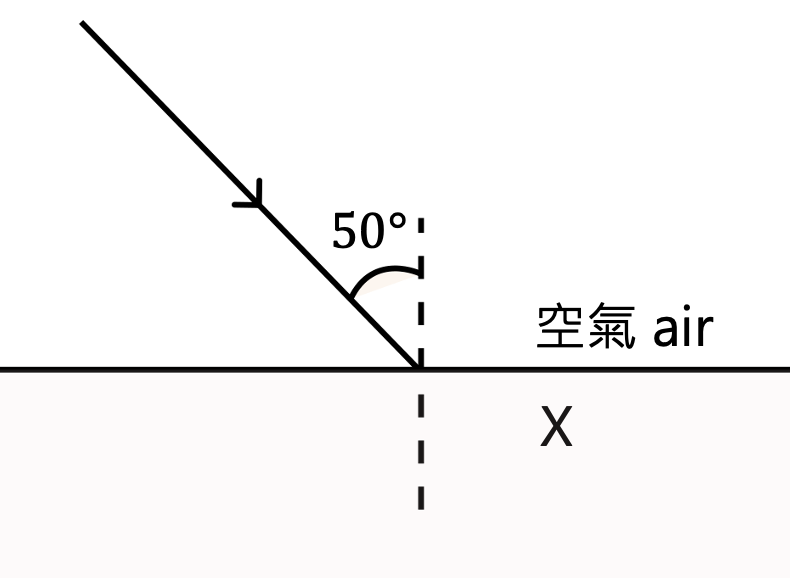
\includegraphics[width=0.45\linewidth]{assets/290132830912ge.png}
    \end{figure}
\end{eg}

\begin{eg}
    圖中是一條光線在三個介質(折射率分別為$n_1$、$n_2$和$n_3$)中的傳播情況。試升序排列$n_1$、$n_2$和$n_3$。\\Figure below shows a ray propagating in between three mediums. The refractive index of mediums are denoted by $n_1$, $n_2$ and $n_3$. Compare their refractive index in ascending order.
    \begin{figure}
        \raggedleft
        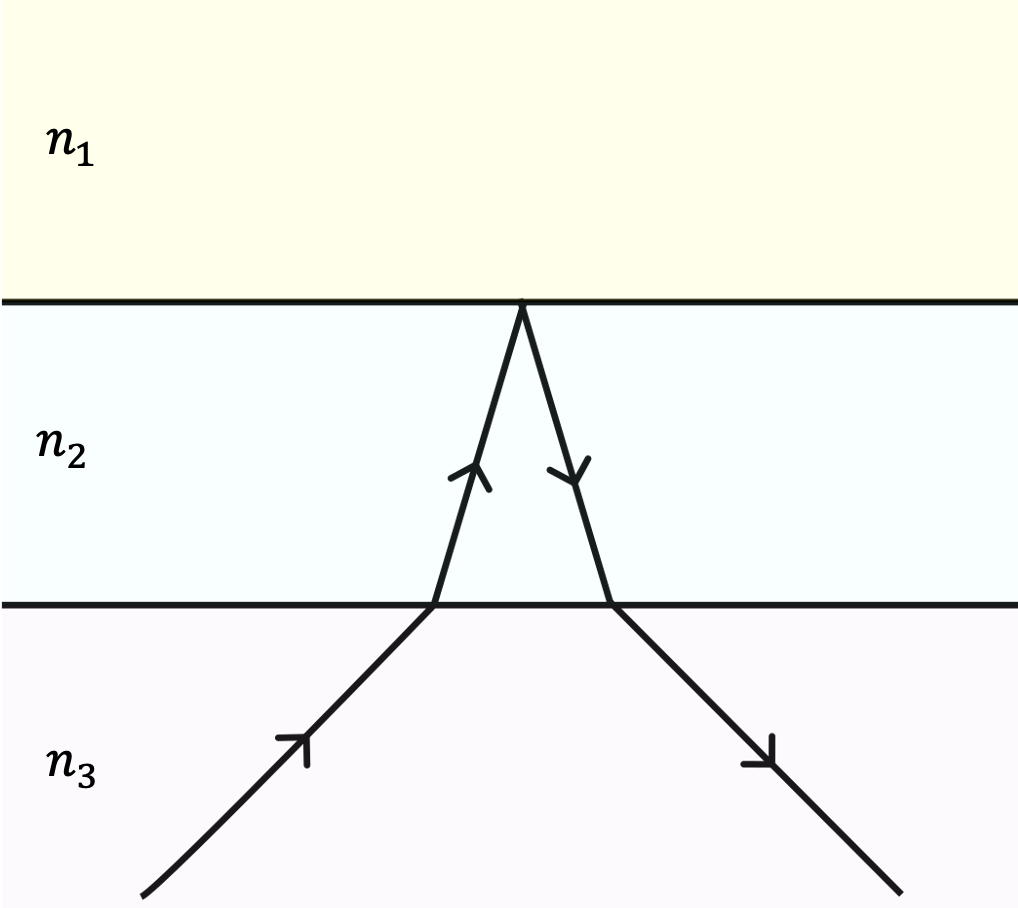
\includegraphics[width=0.4\linewidth]{assets/910991m93.png}
    \end{figure}
\end{eg}

\begin{eg}
一條光線通過一塊長方形玻璃磚。玻璃的折射率為1.50,磚塊的闊 度則為 5 cm。\\A light ray passes through a rectangular block of width 5 cm. The refractive index of the glass is 1.50.
    \begin{figure}
        \centering
        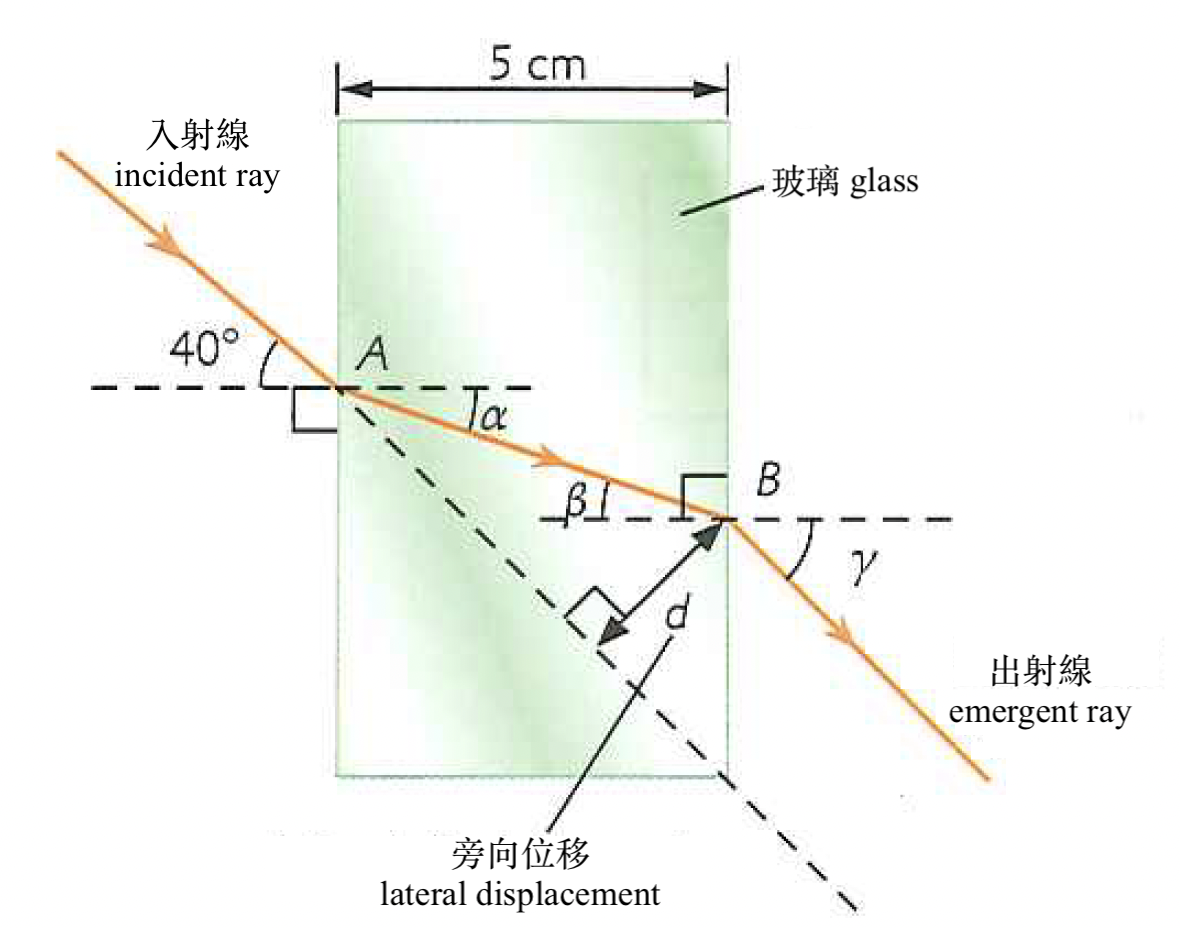
\includegraphics[width=0.6\linewidth]{assets/ud928u82n.png}
    \end{figure}
\end{eg}

\begin{eg}
    \begin{itemize}
        \item [(a)] 求 $\alpha$、$\beta$和$\gamma$。\\Find $\alpha$, $\beta$ and $\gamma$
    \end{itemize}
\end{eg}

\begin{eg}
    \begin{itemize}
        \item [(b)] 求光線的旁向位移$d$。\\Find the lateral displacement $d$ of the light ray.
    \end{itemize}
\end{eg}

\begin{eg}
    \begin{itemize}
        \item [(c)] 若用折射率較高的玻璃磚,光線的旁向位移 $d$ 是增加,減少還是維持不變?\\Does the lateral displacement $d$ increase, decrease or remain unchanged if the block has a larger refractive index?
    \end{itemize}
\end{eg}

\begin{frame}{魚眼視角Fisheye's view}
\begin{columns}
    \column{.5\textwidth}
        {\par\centering
        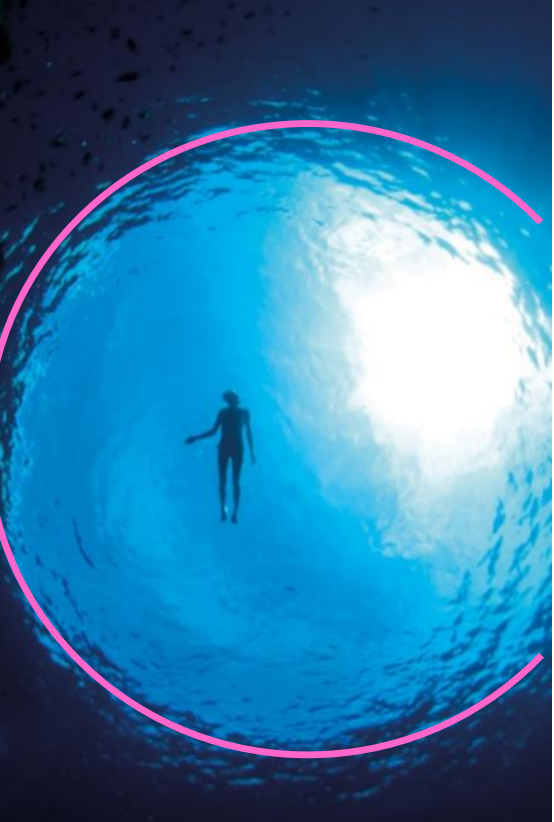
\includegraphics[width=0.75\linewidth]{assets/e1e21d4.png}\par}
    \column{.5\textwidth}
        {\par\centering
        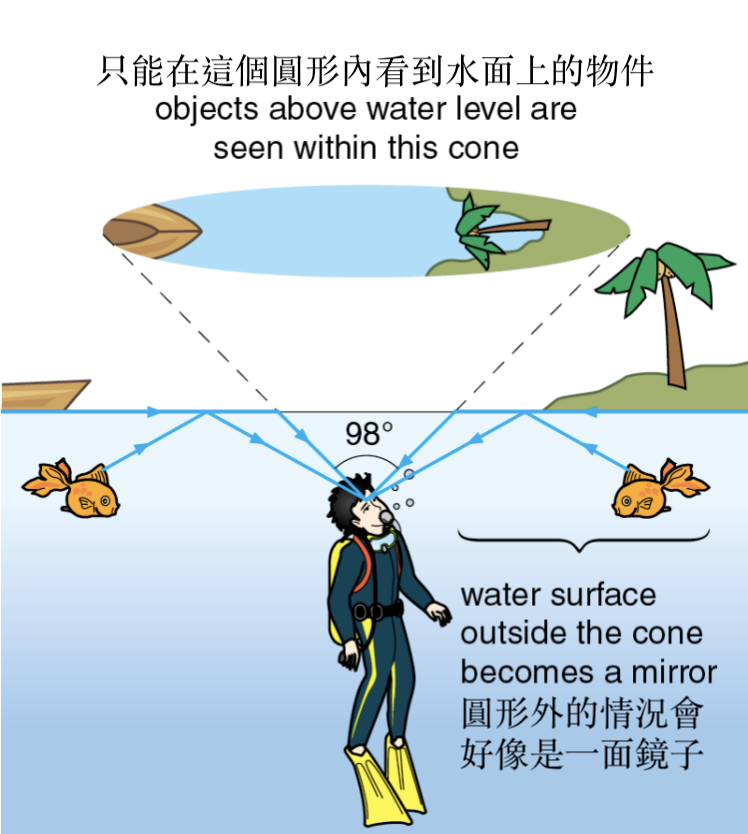
\includegraphics[width=\linewidth]{assets/8jdun98232.png}\par}
\end{columns} 
\end{frame}

\begin{eg}
    一名潛水員從水底向上看。他的眼睛位於水面以下 0.5 m處。(水的折射率=1.33)\\A diver looks upwards from under the water. His eyes are 0.5 m below the surface of the water. (Refractive index of water = 1.33)
    \begin{itemize}
        \item [(a)] 求他所看到的魚眼視角的角度$\theta$。\\Find the angle of the fish-eye view that he sees $\theta$.
    \end{itemize}
    \begin{figure}
        \raggedleft
        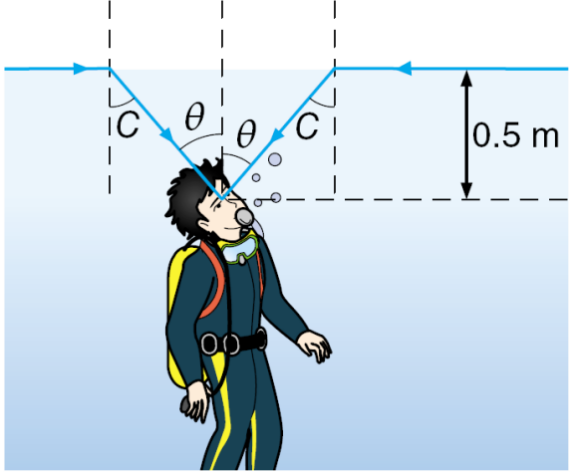
\includegraphics[width=0.35\linewidth]{assets/d980udn34.png}
    \end{figure}

\end{eg}

\begin{eg}
    \begin{itemize}
        \item [(b)] 求對於潛水員,水面視野的直徑。\\Find the diameter of the diver's view.
    \end{itemize}
\end{eg}





















































































\end{document}